\documentclass{article}

\usepackage{hyperref}
\usepackage{graphicx}
\graphicspath{ {./} }

\begin{document}
\title{Project Information Retrieval}
\author{Benjamin Vandersmissen}
\maketitle
\section{Lucene Functionality}
\subsection{Indexing}
A Lucene index consists of documents, each document consists of a number of fields. A field has a unique name for the document, a data type and a value. The supported data types are numerical and Binary points or ranges, textual and even geographical data. The textual types are: String and Text, with the difference being that Text is tokenized and has positional and frequencies indexed, while String only has the document indexed. Other fields can be implemented by the user, by deriving from the Field baseclass.\\

This index is stored as a inverted index, made of posting lists. The index is divided into segments, with a segment containing a subset of the documents and acting as a searchable index over this subset. This index can be written to a directory for easy reuse.\\

For each field, we have a couple options to index it. We can construct a posting list with the documents, documents and frequencies, documents \& frequencies \& positions and last but not least documents \& frequencies \& positions \& offsets.\\

Writing an index is done by using the \textbf{IndexWriter} class, during initialization, one can supply a \textbf{IndexWriterConfig} that has some extra configuration options. One such option is an Analyzer, the Analyzer works on the tokenstream from the documents. It can be used to remove stopwords if you supply the \textbf{DefaultAnalyzer} with a list of stopwords and can also be used to normalize the stream, in case of the \textbf{DefaultAnalyzer}, this means converting every single character to lowercase. \\

Lucene has a lot of other analyzers specifically tuned to various different languages. These are not all included in the core functionality, though they are provided in different modules, such as \textit{analyzers-common} for a lot of special analyzers other than \textbf{StandardAnalyzer}.

Another option is the Similarity measure that will be used, The default used Similarity, is \textbf{BM25Similarity}, Okapi BM 25 with the parameters set to \textit{k1 = 1.2} and \textit{b = 0.75}. Other implemented Similarities include: \textbf{ClassicSimilarity}, which is an implementation of TF-IDF Similarity with tf = \textit{term frequency} and idf = \textit{logarithmic inverse}. Finally we have \textbf{LMDirichletSimilarity} which is an implementation of the mixed Language Model Similarity. Sorting is also an option provided, the index can be sorted on some / all fields in a document, even using custom operators, by using the \textbf{Sort} and \textbf{SortFields} classes.\\

\subsection{Searching}
Lucene has a number of mechanisms to improve the searching for queries. The module \textit{Lucene-suggest} included with the lucene source, implements a Spelling Checker (\textbf{SpellChecker}) and an Auto Complete/Suggest mechanism (\textbf{SuggestIndexSearcher}). To use the spell checking, one needs to supply a Directory with a spelling index in it, the \textbf{SpellChecker} uses Levenshtein distance to calculate the nearest match.\\

Different types of queries are possible : \textbf{TermQuery}, a simple query of one term, \textbf{BooleanQuery} which is a Boolean combination of other Queries. \textbf{WildcardQuery} which uses the wildcards '*', '?' and uses '\textbackslash' as an escape character. And \textbf{PhraseQuery} which is used to exactly match a sequence of terms. PhraseQuery can also be used for proximity search, by using a \textit{slop}, a maximum edit distance for the phrase. \\

Lucene also introduces a \textbf{QueryParser} in the module \textit{Lucene-queryparser}, this parser transforms a string representation of a query in the correct Lucene objects. This parser only works with one field, this means that a plaintext query will be transformed to a Lucene query for the specified field only. If one wants to parse a query over multiple fields, the class \textbf{MultiQueryParser} can be used.\\

Executing a query is done by using \textbf{IndexSearcher}.search method, this method returns a \textbf{TopDocs} instance which contains the total number of hits and the documents matching the query, sorted on descending score.

\section{Benchmarking}
\subsection{Code and Executable}
The code necessary for building and running the application is on github : \url{https://github.com/Benjamin-Vandersmissen/ProjectIR}. Libraries included are Lucene and a couple of modules for Lucene. A compiled executable will be provided as well. \textbf{This executable is compiled using java openjdk 11.05, the default for ubuntu 18.04!}

\subsection{Data files}
The data files used in the benchmarking are derived from the dataset of Stackoverflow questions, though they are not the same as the preprocessed dataset, this one was preprocessed by myself. I tried to be as faithful as possible to the restrictions on the preprocessed one, with the tags for example, but there is one extra additition not present in the preprocessed files, at least to my knowledge. The XML file is encapsuled in the $<$file$>$ tag, otherwise the default java XML parser would complain and wouldn't parse the XML files.

\subsection{Index Construction}
The XML files are converted to a Lucene indexable \textbf{Document} in the following way: the document has a field \textit{title}, which is the title of the question, it is stored in the index, but not indexed i.e. it can't be searched on. It is stored in the index to easily test for the ground truth. The next field is \textit{question} it contains the question body and is a TextField, which means it is tokenized and the positions as well as the frequencies for each document are indexed. The fields \textit{tags} and \textit{answers} are also TextFields, indexing the tags resp. a concatenation of the answer bodies. A field \textit{id} is also included, stored but not indexed, for convenience sake. This field directly refers to the file of the question.\\

By using the whitespace analyser, special characters are ignored. Code fragments are not removed while processing the xml files, which means they are indexed as well.

\subsection{Ground Truth}
The ground truth is done by labeling each document with the title in the index, without indexing the title itself. Constructing a query containing only the title should return the document somewhere in the top documents, this should be easily tested by comparing the query to the titles of the first \textit{k} documents. One of the parameters we need to balance is \textit{k}, if we make \textit{k} too small, it is possible that we have a lot of false negatives, make \textit{k} too high and we introduce a lot of false positives.\\

There are different possibilities to evaluate this ground truth. For example, we can use a simple boolean measure and calculate the percentage the document occurs in the top \textit{k} documents. This measure could then be used akin to precision.\\

For example: if for 60\% of queries, we succesfully retrieve the relevant document in the top-10 documents, we have a precision of 10\% in 60\% of the cases which means in 40\% of the cases we have a precision of 0\%.
Which means we have an average precision of 6\% for returning the top 10 documents for a given setup. This reasoning is only sound if we have a large enough sample for the dataset and if we assume only one document is ever relevant.\\ 

Another possibility lies in using the score of the documents in the retrieval to evaluate the performance. If the labeled document has a higher score, then the retrieval method should be better. In this benchmark, we use the first evaluation method discussed.\\

We consider the first 1000 documents as a test set for the information retrieval. For each document, we save the title and use the title as a search query. Then we use the query to search the index and return the top-k documents for the query. If one of the returned documents has the same title as the query, then we know that this is the same document. These 1000 documents account for around 0.05 \% of the total set of documents.

\subsection{Approach}
We will compare the results for benchmarks with a number of different parameters. The first parameter we will vary is \textit{fields}, which fields do we use for searching. There are two possibilities here, searching on the question body only or searching on all fields.\\

The Similarity used is another parameter, we will compare each of the three main similarities seen during the course: Vector Space Model (\textbf{ClassicSimilarity}), Okapi BM25 (\textbf{BM25Similarity}) and Language Mixture Model (\textbf{LMDirichletSimilarity})\\

Lastly we will vary the preprocessing used. There are once again two options; no preprocessing used at all, and making all tokens lowercase.\\

We will study each possible combination for these three parameters, in total 12 different combinations. The evaluation will be done using the approach mentioned in the section above, for three different values of \textit{k}, being \textit{k=10}, \textit{k=50}, \textit{k=100}.

\section{Querying One field}
The specific field queried is the \textit{question} field, which contains the body of the question asked on stack overflow. One might assume that when searching for a specific question using the title, the question body is the most relevant to the title, so this is the approach we use first.

\subsection{Okapi BM25 Similarity}
The following benchmarks use the default similarity : \textbf{BM25Similarity}. See section \textbf{Lucene Functionality} for more information.
\subsubsection{No Preprocessing}
We use the whitespaceAnalyzer in this benchmark, which creates the tokens purely by splitting the query and the documents on whitespaces and doesn't preprocess any more. \\
Benchmarking with the parameters k=10, k=50 and k=100 yield the following results:\\

\begin{center}
\begin{tabular}{|c|c|c|} \hline
\textbf{k} & \textbf{documents found} & \textbf{precision}\\ \hline
10 & 251 & 2.51\%\\
50 & 341 & 0.68\%\\
100 & 380 & 0.38\%\\ \hline
\end{tabular}
\end{center}
\subsubsection{Lower case normalization}
The only change with the previous benchmark, is the use of a tokenfilter, each token is normalized by making all characters lowercase.

\begin{center}
\begin{tabular}{|c|c|c|} \hline
\textbf{k} & \textbf{documents found} & \textbf{precision}\\ \hline
10 & 303 & 3.03\%\\
50 & 403 & 0.81\%\\
100 & 446 & 0.45\%\\ \hline
\end{tabular}
\end{center}

\subsection{TF-IDF Similarity}
This section uses the \textbf{ClassicSimilarity}, the legacy Lucene default, a implementation of TF-IDF weighting.
\subsubsection{No Preprocessing}
\begin{center}
\begin{tabular}{|c|c|c|} \hline
\textbf{k} & \textbf{documents found} & \textbf{precision}\\ \hline
10 & 178 & 1.78\%\\
50 & 266 & 0.53\%\\
100 & 320 & 0.32\%\\ \hline

\end{tabular}
\end{center}

\subsubsection{Lower case normalization}
\begin{center}
\begin{tabular}{|c|c|c|} \hline
\textbf{k} & \textbf{documents found} & \textbf{precision}\\ \hline
10 & 221 & 2.21\%\\
50 & 323 & 0.65\%\\
100 & 372 & 0.37\%\\ \hline

\end{tabular}
\end{center}

\subsection{Language Mixture Models}
This section uses the \textbf{LMJelineMercerSimilarity}, a language mixture model with lambda=0.5.
\subsubsection{No Preprocessing}
\begin{center}
\begin{tabular}{|c|c|c|} \hline
\textbf{k} & \textbf{documents found} & \textbf{precision} \\ \hline
10 & 262 & 2.62\%\\
50 & 340 & 0.68\%\\
100 & 391 & 0.39\%\\ \hline

\end{tabular}
\end{center}

\subsubsection{Lower case normalization}
\begin{center}
\begin{tabular}{|c|c|c|} \hline
\textbf{k} & \textbf{documents found} & \textbf{precision}\\ \hline
10 & 318 & 3.18\%\\
50 & 414 & 0.83\%\\
100 & 457 & 0.46\%\\ \hline

\end{tabular}
\end{center}

\subsection{Plot}
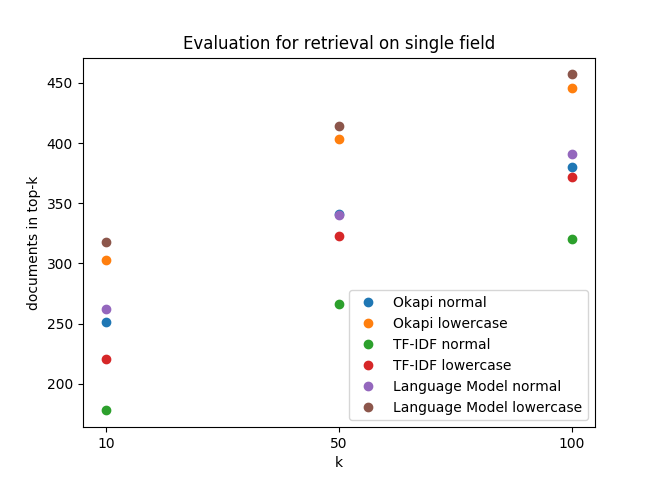
\includegraphics[width=\textwidth]{one_field}

\section{Querying all fields}
When we want to use queries other than the title, it might be more useful to consider all the fields in a document. When searching documents on title, the effect can be twofold, for one, the answers could contain some terms from the title not occuring in the question body, but on the other hand, this could negatively impact the score by increasing the length of the document needlessly. However, if we assume the title of a question accurately describes the question body, then it would be wise to only search in the question body, still, it is worth to consider all the options.

\subsection{Okapi BM25 Similarity}
\subsubsection{No Preprocessing}
\begin{center}
\begin{tabular}{|c|c|c|} \hline
\textbf{k} & \textbf{documents found} & \textbf{precision}\\ \hline
10 & 199 & 1.99\%\\
50 & 296 & 0.59\%\\
100 & 342 & 0.34\%\\ \hline
\end{tabular}
\end{center}
\subsubsection{Lower case normalization}

\begin{center}
\begin{tabular}{|c|c|c|} \hline
\textbf{k} & \textbf{documents found} & \textbf{precision}\\ \hline
10 & 244 & 2.44\%\\
50 & 349 & 0.70\%\\
100 & 408 & 0.41\%\\ \hline
\end{tabular}
\end{center}

\subsection{TF-IDF Similarity}
\subsubsection{No Preprocessing}
\begin{center}
\begin{tabular}{|c|c|c|} \hline
\textbf{k} & \textbf{documents found} & \textbf{precision}\\ \hline
10 & 159 & 1.59\%\\
50 & 244 & 0.49\%\\
100 & 297 & 0.30\%\\ \hline

\end{tabular}
\end{center}

\subsubsection{Lower case normalization}
\begin{center}
\begin{tabular}{|c|c|c|} \hline
\textbf{k} & \textbf{documents found} & \textbf{precision}\\ \hline
10 & 187 & 1.87\%\\
50 & 288 & 0.57\%\\
100 & 350 & 0.35\%\\ \hline

\end{tabular}
\end{center}

\subsection{Language Mixture Models}
\subsubsection{No Preprocessing}
\begin{center}
\begin{tabular}{|c|c|c|} \hline
\textbf{k} & \textbf{documents found} & \textbf{precision}\\ \hline
10 & 221 & 2.21\%\\
50 & 306 & 0.61\%\\
100 & 360 & 0.36\%\\ \hline

\end{tabular}
\end{center}

\subsubsection{Lower case normalization}
\begin{center}
\begin{tabular}{|c|c|c|} \hline
\textbf{k} & \textbf{documents found} & \textbf{precision}\\ \hline
10 & 266 & 2.66\%\\
50 & 359 & 0.72\%\\
100 & 411 & 0.41\%\\ \hline
\end{tabular}
\end{center}

\subsection{Plot}

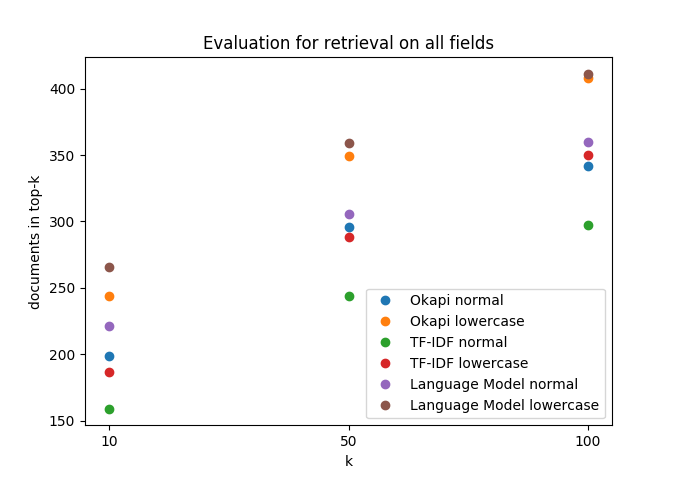
\includegraphics[width=\textwidth]{all_fields}

\section{Benchmarking Conclusions}
We can infer the following conclusions from the raw data. 

Firstly, if we have the title of a document as query, it is beneficial to only search in the question body. On average 39 extra documents are found per benchmark, though the effect is lesser with Tf-Idf. This could be explained, if we assume that a question title is more intensely related to a question body than to the answers on the question.\\

From the data, we can conclude that from the three different similarities, the language mixture model is narrowly better than Okapi, with Tf-Idf being a distant third. Tweaking the parameters of Okapi and the Language mixture might increase the performance of both.\\

The last conclusion is the difference between Truecase and lowercase documents and queries. We can clearly see in the data that converting the documents to all lowercase is beneficial for the queries. Using lowercase documents leads to an average of 54 more documents found, with most of them being in the top-10 documents.\\

For the k-values we have compared and the assumption that there is only one relevant document, it is always preferred to pick k=10 for the best precision.\\

Since the setup with the Language mixture model with lowercase similarity and searching over the question body gave the best result in our benchmarks, this is the default setting in the search engine.

\newpage

\section{Relevance Feedback}
\subsection{Rocchio Algorithm}
Relevance Feedback has been implement using the Rocchio algorithm. This algorithm functions in conjunction with the Vector Space Model. A vector representation of a query is a weighted average of the original query, the average of the set of the relevant documents and the negative average of the set of the irrelevant documents. This type of Relevance Feedback is active, this means the user needs to mark the (ir)relevant documents instead of the computer determining the relevant documents.

\subsection{Demonstration}
Using the benchmarking dataset and the query "test java", we get the following results.

\begin{center}
\begin{tabular}{|c|c|c|} \hline
\textbf{pos} & \textbf{title} & \textbf{Relevant?} \\ \hline \hline
1 & can we use java code in web2py application code? & No \\ \hline
2 & Tool to convert Java source to C++ source & Yes \\ \hline
3 & Linking in test libraries with CppUnit & Yes \\ \hline
4 & What is the Windows registered class of a Java window? & No \\ \hline
5 & C++ Updating a data member using a struct pointer & Yes \\ \hline
6 & Difference between build /clean \& build in a & \\ & c++ project in netbeans IDE,test and debug test & Yes \\ \hline
7 & Using funcarg value in pytest\_generate\_tests function & No \\ \hline
8 & Using CppUnit for memory leak detection & Yes \\ \hline
9 & Java reflection: create a instance using params  & \\ & from a treemap like python & No \\ \hline
10 & AppEngine: Running Python code on the fly & No \\ \hline
\end{tabular}
\end{center}

We have marked all the documents with titles pertaining to C++ as relevant, after relevance feedback, we get the following results:\\

\begin{center}
\begin{tabular}{|c|c|} \hline
\textbf{pos} & \textbf{title} \\ \hline \hline
1 & Linking in test libraries with CppUnit \\ \hline
2 & Tool to convert Java source to C++ source \\ \hline
3 & C++ Updating a data member using a struct pointer \\ \hline
4 & Difference between build /clean \& build in a c++ project \\ & in netbeans IDE,test and debug test \\ \hline
5 & Using CppUnit for memory leak detection \\ \hline
6 & Using funcarg value in pytest\_generate\_tests function \\ \hline
7 & native unit test, debugger performing a remote \\ & operation that is taking longer than expected \\ \hline
8 & can we use java code in web2py application code? \\ \hline
9 & How does gtest compare the values in two arrays? \\ \hline
10 & Writing tests for stochastic functions \\ \hline
\end{tabular}
\end{center}

We can clearly see that C++ related questions have been pushed up in the new top 10. In fact, only two of the questions in the updated top 10 are related to Java, in contrast to the 4 from the original top 10.

\subsection{Evaluation}
We can base our evaluation on the same principles of the benchmarking, by measuring the percentage a query returns the correct document in the top-k results. We will compare the results without feedback expansion to the results  after one round of feedback expansion. Because this implementation is very time consuming, we construct our index out of 5000 documents.\\

Two documents will be considered relevant to the other if their title contains at least two terms of the query. This is done in order to make the benchmarking be autonomous, but is of course not a perfect replacement for user-based evaluation. Though a user might employ a similar reasoning in selecting the relevant documents. \\

\textbf{These results cannot be compared with the results from the previous section!} This is due to the fact these results were obtained on a small subset of the total documents. Returning the top 10 is +/- 0.0005\% of the total index, but +/- 0.2\% for the subset. If we would want comparable precentages, we should return the 0.025 top-scoring documents, which is of course impossible. \\

The first three benchmarks will be with gamma=0, this is to emulate the fact that modern search engines follow the same approach. Aftwerwards, we will do the same tests again, but with a constant low gamma, to compare them and see if there are merits in setting a low gamma. We will then compare the method to the default to see if there are any notable gains by using relevance feedback. 

\subsection{Results}

\subsubsection{Results with no Relevance feedback}
This is the result of pure vector space model. We will use these results as a control group for the relevance feedback.

\begin{center}
\begin{tabular}{|c|c|} \hline
\textbf{k} & \textbf{documents returned} \\ \hline
10 & 425\\
50 & 572\\
100 & 638\\ \hline
\end{tabular}
\end{center}

\subsubsection{Alpha=0.5, Beta=0.5, Gamma=0}

\begin{center}
\begin{tabular}{|c|c|} \hline
\textbf{k} & \textbf{documents returned} \\ \hline
10 & 427 \\
50 & 584\\
100 & 653\\ \hline
\end{tabular}
\end{center}

\subsubsection{Alpha=0.7, Beta=0.3, Gamma=0}

\begin{center}
\begin{tabular}{|c|c|} \hline
\textbf{k} & \textbf{documents returned} \\ \hline
10 & 429\\
50 & 583\\
100 & 653\\ \hline
\end{tabular}
\end{center}

\subsubsection{Alpha=0.9, Beta=0.1, Gamma=0}

\begin{center}
\begin{tabular}{|c|c|} \hline
\textbf{k} & \textbf{documents returned} \\ \hline
10 & 431\\
50 & 585\\
100 & 650\\ \hline
\end{tabular}
\end{center}

\subsubsection{Alpha=0.5, Beta=0.5, Gamma=0.1}

\begin{center}
\begin{tabular}{|c|c|} \hline
\textbf{k} & \textbf{documents returned} \\ \hline
10 & 425\\
50 & 583\\
100 & 652\\ \hline
\end{tabular}
\end{center}

\subsubsection{Alpha=0.7, Beta=0.3, Gamma=0.1}

\begin{center}
\begin{tabular}{|c|c|} \hline
\textbf{k} & \textbf{documents returned} \\ \hline
10 & 428\\
50 & 583\\
100 & 654\\ \hline
\end{tabular}
\end{center}

\subsubsection{Alpha=0.9, Beta=0.1, Gamma=0.1}

\begin{center}
\begin{tabular}{|c|c|} \hline
\textbf{k} & \textbf{documents returned} \\ \hline
10 & 424\\
50 & 582\\
100 & 646\\ \hline
\end{tabular}
\end{center}

\subsection{Conclusions}
When we compare the relevance feedback results to the control group, we can see that there is noticeable improvement independent for all tested combinations of parameters. This improvement is much more pronounced with a higher \textit{k} value. At \textit{k} = 10, the difference is almost non-existent, but at \textit{k} = 50 or 100, there is a more pronounced difference, with around 10 extra matching documents found per benchmark.\\

Using gamma=0.1 instead of gamma=0, doesn't really improve the results, if anything, it has a slightly worse performance than the equivalent benchmark with no negative feedback. This can be seen in the benchmarks with alpha=0.9 and beta=0.1.\\ 

If we employ the same reasoning to estimate the precision, we have around a 0.02\% increase in precision at \textit{k}=50 and a 0.01\% increase in precision at \textit{k} = 100. We can estimate the recall as well, by using the same idea as with the precision. If we get the correct document in 60\% of the cases and we assume only one document is relevant, then our recall is 100\% in those 60\% of the tests and 0\% in the other tests, so our estimated recall is  60\%.\\

In the final version we use the parameters alpha=0.9, beta=0.1, gamma=0, because they gave the best results during our benchmark.\\  
\end{document}